% Build with latexmk -pdf Beat2Body_Proposal.tex (requires IEEEtran and PGF/TikZ).
\documentclass[conference,letterpaper]{IEEEtran}
\usepackage[T1]{fontenc}
\usepackage{amsmath}
\usepackage{booktabs}
\usepackage{balance}
\usepackage{cite}
\usepackage{microtype}
\usepackage{tikz}
\usetikzlibrary{arrows.meta}
\usepackage[hidelinks]{hyperref}

\definecolor{motionblue}{HTML}{27517C}
\definecolor{audioteal}{HTML}{246C63}
\definecolor{inkgray}{HTML}{424B53}
\hypersetup{
  pdftitle={Beat2Body: Music- and Genre-Conditioned 2D Dance Generation},
  pdfauthor={YinHsuan Hsu, Yi Xin, Sizhe Zhang},
  pdfsubject={ELEC/COMP 576 Final Project Proposal}
}

\title{Beat2Body: Music- and Genre-Conditioned\\2D Dance Generation}
\author{\IEEEauthorblockN{YinHsuan Hsu, Yi Xin, and Sizhe Zhang}
\IEEEauthorblockA{ELEC/COMP 576 -- Introduction to Deep Learning\\
Final Project Proposal $\cdot$ November 19, 2026}}

\begin{document}
\maketitle

\begin{abstract}
Choreographers, animators, and game developers need dance motion that fits a given piece of music and style, but recording it with motion capture is expensive. We propose Beat2Body, a deep generative model that takes a music excerpt and one of ten dance genres and generates a 2D skeleton sequence that moves with the rhythm. Unlike prior music-to-dance systems trained on studio 3D motion capture, Beat2Body learns from 2D joint tracks extracted from ordinary single-camera video: 1,410 videos (5.2 hours) of the AIST Dance Video Database processed with three pose estimators. We adapt the EDGE diffusion transformer to image-plane motion and add losses for body-size stability and rhythmic energy. Preliminary results expose the central difficulty: a first model produced realistic poses but moved at half the real speed, while an energy loss restored real-dancer speed and halved the kinetic Fr\'echet distance on held-out songs at the cost of body-size stability. We will run controlled ablations of losses, training recipe, model size, and pose estimator against a recurrent baseline, and evaluate realism, rhythm, genre, and stability on songs never seen in training.
\end{abstract}

\begin{IEEEkeywords}
music-to-dance generation, diffusion models, 2D pose, rhythm, genre conditioning
\end{IEEEkeywords}

\section{Background and Motivation}
Creating dance for a new track involves choosing steps and gestures, timing accents to the music, and connecting them into phrases. Even professional dancers run short of ideas when improvising to unfamiliar music, and few are fluent in many genres. Choreographers could use a generator to audition several interpretations before rehearsing; animators and game studios, which need large amounts of character dance, could block motion against a soundtrack without a motion-capture session.

\textbf{Problem statement.} Given a music excerpt and one of ten genre labels, generate the 2D positions of 17 body joints (nose, shoulders, elbows, wrists, hips, knees, ankles, and so on) at 30 frames per second, such that the motion (i) looks like real dancing, (ii) moves with the beat, (iii) shows the requested genre, and (iv) keeps stable body proportions over a 20-second excerpt. One track admits many valid dances, so closeness to one reference performance is a poor measure of quality; we evaluate pose, dynamics, rhythm, and style separately.

\textbf{Background.} Two deep-learning tools make this possible. \emph{Pose estimators} are neural networks that locate body joints in each video frame, turning video into skeleton tracks \cite{yang2023,cao2021,bazarevsky2020}. \emph{Diffusion models} generate data by learning to remove noise: during training, noise is added to real motion and a network learns to recover the clean motion; during generation, the network starts from random noise and removes it step by step, guided by the music and genre \cite{song2021}.

\textbf{Prior work and gap.} Lee \emph{et al.} generated 2D dance for three genres by composing movement units from web videos \cite{lee2019}. Later systems moved to 3D motion capture: the FACT transformer on AIST++ \cite{li2021} and the EDGE diffusion model, which added a foot-contact penalty and long-form generation \cite{tseng2023}; recent work models beats explicitly in 3D diffusion \cite{gao2026} or maps 2D poses into image latents \cite{dancedit}. The 3D systems depend on data reconstructed in a nine-camera studio, which is unavailable for most dancers and styles. Learning from single-camera video would open far more footage, but its labels are noisy, projected limb lengths change with the viewpoint, and depth is lost. How modern diffusion models handle rhythm in this setting, and how the choice of pose estimator affects the generator, have not been studied: our pilot shows that a 2D diffusion model reproduces poses but suppresses beat-level movement.

\textbf{Proposed contributions.} (1) A 2D adaptation of EDGE with dancer-level scaling and a projected bone-length loss; (2) a smoothed, timing-invariant energy loss and a beat-band power metric for rhythmic movement; (3) beat-relative attention and separate music and genre guidance, tested by shifting the beat grid and swapping the track or genre; (4) a controlled comparison of three pose estimators as training data; and (5) an evaluation on held-out songs with rhythm and genre controls.

\section{Proposed Experimentation and Implementation}

\subsection{Dataset}
We use the front camera (\texttt{c01}) of the AIST Dance Video Database \cite{tsuchida2019}, free for academic research through its official download \cite{aistdownload}: 210 advanced performances (each dancer's own choreography, about 35\,s) and 1,200 basic dances (ten genre-basic routines per dancer, each performed to four songs, 7--12\,s), set to 60 songs in ten genres (ballet jazz, break, house, krump, LA hip-hop, lock, middle hip-hop, pop, street jazz, waack). The 1,410 videos total 5.2 hours, the size of AIST++. Our processed tracks and features are public \cite{beat2bodydata}.

Videos are resampled to 30\,fps. DWPose, OpenPose, and MediaPipe's BlazePose landmarks are mapped to the COCO-17 joint order (OpenPose and MediaPipe for the advanced dances); low-confidence joints and isolated jumps are removed, short gaps interpolated, and jitter smoothed with a Savitzky--Golay filter, with a mask recording observed joints. Joints are centred on the hip midpoint, which is kept as a root trajectory, and both are divided by the dancer's median torso length over all of that dancer's videos (a per-video median enlarged dancers two- to threefold in break floor routines). Each frame holds 34 joint coordinates, two root coordinates, and two ankle-contact flags. Music features at 30\,Hz are EDGE's 35 features (onset strength, cepstral coefficients, chroma, beat indicators) plus the sine and cosine of the beat phase. Because the beat tracker chose the wrong tempo for 10 of 60 songs \cite{beat2bodyprogress}, beats follow the published AIST tempo.

One song per genre is held out entirely as the test set (Table~\ref{tab:split}); the remaining videos are split into training and validation by video, and the tempo versions of each basic routine stay in one partition. Clips are eight-second windows at two-second strides; the model trains on five-second crops. An audit of labels, lengths, beats, and splits passes on all 4,824 clips.

\begin{table}[t]
\caption{DWPose split: advanced subset / all 1,410 videos}
\label{tab:split}
\centering
\begin{tabular}{lrrr}
\toprule
Partition & Videos & Clips & Songs \\
\midrule
Training & 145 / 1,013 & 2,155 / 3,423 & 50 / 50 \\
Validation & 29 / 161 & 440 / 632 & 24 / 50 \\
Held-out-song test & 36 / 236 & 489 / 769 & 10 / 10 \\
\bottomrule
\end{tabular}
\end{table}

\subsection{Design requirements}
\begin{itemize}
\item \emph{Function:} accept a music file and a genre label; export joint coordinates and a synchronized stick-figure video for at least 20\,s.
\item \emph{Realism:} lower kinetic and pose Fr\'echet distances than the recurrent baseline; kinetic diversity within 25\% of real dancers.
\item \emph{Rhythm:} mean joint speed and 1--4\,Hz beat-band power within 25\% of real; movement accents concentrated on the beat more than on shifted beat grids.
\item \emph{Stability:} torso-length variation over a 20\,s excerpt within 15\% of real; foot-sliding proxy within 25\% of real.
\item \emph{Genre:} requested genre recognized by a classifier trained on real motion well above chance (10\%).
\item \emph{Efficiency:} each training run within two hours on one 24\,GB GPU.
\end{itemize}

\subsection{Architecture}
\textbf{Baseline.} An autoregressive gated recurrent unit (GRU) predicts the next frame from the previous frame, a temporal convolution over the audio, and a learned genre embedding; at generation time it feeds back its own predictions.

\textbf{Main model.} A 2D adaptation of EDGE \cite{tseng2023} (Fig.~\ref{fig:method}). A two-layer transformer encodes the music; an eight-layer transformer decoder (46.9M parameters; 7.1M in a four-layer variant for ablations) attends to the noisy five-second motion window and, through cross-attention, to the music, conditioned on the noise level and genre. Music and genre are each dropped with probability 0.25 during training to enable classifier-free guidance. We use 1,000 noise levels, 50-step DDIM sampling \cite{song2021}, and half-overlapping windows for 20-second dances. The loss combines EDGE's reconstruction, velocity, joint-position, and foot-contact terms with (a) a projected bone-length loss that matches each bone's on-screen length to the same bone in the reference frame, allowing natural foreshortening, and (b) an energy term on the log ratio of each joint's smoothed speed and movement amplitude to the reference window, which does not depend on the exact timing of accents. Training uses 1,000 warm-up updates, gradient clipping, cosine learning-rate decay, and the checkpoint with the lowest validation loss.

\begin{figure}[t]
\centering
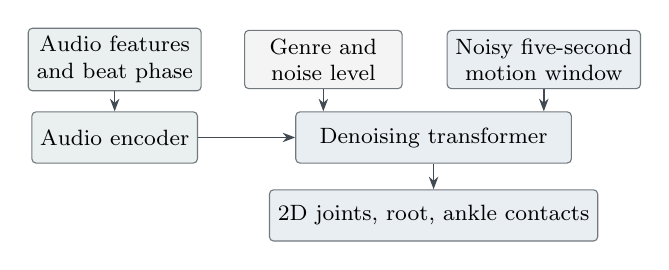
\begin{tikzpicture}[
  x=1cm,y=1cm,font=\footnotesize,
  block/.style={draw=inkgray!75,rounded corners=1.5pt,align=center,
    minimum height=0.65cm,inner sep=3pt,fill=inkgray!6},
  edge/.style={-{Stealth[length=1.6mm]},line width=.55pt,draw=inkgray}
]
  \node[block,fill=audioteal!10,minimum width=2.06cm] (audio) at (0,1.96) {Audio features\\and beat phase};
  \node[block,minimum width=2.00cm] (genre) at (2.65,1.96) {Genre and\\noise level};
  \node[block,fill=motionblue!10,minimum width=2.11cm] (noise) at (5.45,1.96) {Noisy five-second\\motion window};
  \node[block,fill=audioteal!10,minimum width=2.06cm] (enc) at (0,.97) {Audio encoder};
  \node[block,fill=motionblue!10,minimum width=3.50cm] (decoder) at (4.05,.97) {Denoising transformer};
  \node[block,fill=motionblue!10,minimum width=3.50cm] (output) at (4.05,-.02) {2D joints, root, ankle contacts};
  \draw[edge] (audio) -- (enc);
  \draw[edge] (enc) -- (decoder);
  \draw[edge] (genre) -- (genre |- decoder.north);
  \draw[edge] (noise) -- (noise |- decoder.north);
  \draw[edge] (decoder) -- (output);
\end{tikzpicture}
\caption{One denoising step. The decoder uses cross-attention to the encoded music and conditions on the requested genre and current noise level.}
\label{fig:method}
\end{figure}

\begin{table*}[t]
\caption{Step-by-step plan, measures of success, and leads}
\label{tab:plan}
\centering
\begin{tabular}{@{}p{.95in}p{.55in}p{2.55in}p{1.95in}p{.85in}@{}}
\toprule
Stage & Time & Work & Measure of success & Lead \\
\midrule
1. Data & Done & 2D dataset: 1,410 videos, three pose estimators, beat-aligned music features, held-out-song split. & Audit passes on all 4,824 clips; test songs disjoint from training. & YinHsuan Hsu \\
\addlinespace[2pt]
2. Baseline & Week 1 & Train the GRU on the full dataset. & Complete 20\,s rollouts; all metrics logged as the reference bar. & Sizhe Zhang \\
\addlinespace[2pt]
3. Diffusion ablations & Weeks 1--2 & Losses vs.\ recipe vs.\ size; loss rebalancing; regularization components one at a time. & Speed and beat-band power within 25\% of real, torso variation within 15\%, FD$_p$ within 20\% of Model A. & Sizhe Zhang \\
\addlinespace[2pt]
4. Model design experiments & Weeks 2--3 & Separate music and genre guidance; beat-relative cross-attention; kinematic skeleton decoder; phrase planning (each only if the previous step leaves its target unmet). & Accents follow a shifted beat grid at unchanged beat-band power; motion responds to the track and genre; torso within 15\%; fewer repeated moves over 20\,s. & Sizhe Zhang \\
\addlinespace[2pt]
5. Data and pose-tool study & Weeks 2--3 & Advanced-only vs.\ all videos; DWPose vs.\ OpenPose vs.\ MediaPipe on matched windows. & Rankings whose differences exceed the spread across seeds. & YinHsuan Hsu \\
\addlinespace[2pt]
6. Held-out evaluation & Week 3 & Locked settings; test songs; timing test; genre classifier. & Main model beats GRU on FD$_k$, FD$_p$, and timing; genre accuracy well above 10\%. & Yi Xin \\
\addlinespace[2pt]
7. Demo and report & Week 4 & Music-file input, 20\,s videos with sound, report and poster. & End-to-end demo on a new track; documented failure cases. & All members \\
\bottomrule
\end{tabular}
\end{table*}

\subsection{Preliminary results}
We trained 7.1M-parameter diffusion models on cloud GPUs (Table~\ref{tab:pilot}). Model A, with per-video scaling and the bone-length loss, produced the most realistic poses and a stable torso, but moved at 53\% of the real speed with 24\% of the real movement in the 1--4\,Hz band (Fig.~\ref{fig:power}), on training and validation music alike, so the problem is not overfitting. Standardizing the motion features with $v$-prediction \cite{salimans2022} destroyed pose quality, and an energy loss on raw speed was partly met with jitter. Run 2.1 (smoothed energy loss, all 1,410 videos) restored real-dancer speed; on the 769 held-out-song windows it halved the kinetic distance of Model A (22.5 vs.\ 43.7) and raised kinetic diversity from 2.5 to 7.1 (real: 7.4), but its pose distance rose from 34.6 to 41.8 and its torso varied twice as much as real (0.223 vs.\ 0.105). Fig.~\ref{fig:pose} shows Model A's restrained movement next to the recorded dancer. These results define the trade-off the proposed experiments must resolve.

\begin{table}[t]
\caption{Diffusion models (7.1M) on advanced validation windows}
\label{tab:pilot}
\centering
\setlength{\tabcolsep}{3.2pt}
\begin{tabular}{lrrrrrr}
\toprule
Model & FD$_k$\,$\downarrow$ & FD$_p$\,$\downarrow$ & Foot\,$\downarrow$ & Speed & Beat & Torso \\
\midrule
First run & 52.8 & 55.5 & 0.048 & 0.58 & -- & 0.134 \\
Model A & 43.7 & \textbf{23.1} & \textbf{0.038} & 0.53 & 0.24 & \textbf{0.111} \\
Regularized & 46.5 & 46.6 & 0.063 & 0.57 & 0.20 & 0.157 \\
+ z-score, $v$ & 974 & 69.1 & 0.075 & 1.06 & 0.26 & 0.047 \\
+ energy (raw) & 327 & 37.0 & 0.076 & 0.80 & 0.33 & 0.077 \\
Run 2.1 & \textbf{36.9} & 67.3 & 0.054 & 1.19 & 1.71 & 0.186 \\
\midrule
Real & 0 & 0 & 0.029 & 1.00 & 1.00 & 0.103 \\
\bottomrule
\end{tabular}

\vspace{2pt}
\begin{minipage}{\columnwidth}
\footnotesize 440 five-second windows. FD: Fr\'echet distance of kinetic and pose features. Speed and Beat (1--4\,Hz power, BeatPow): ratios to the real windows. Torso: standard deviation over mean of torso length in ten 20-second generations. The ablations trained 20,000 updates on advanced dances; Run 2.1 trained 30,000 on all videos.
\end{minipage}
\end{table}

\begin{figure}[t]
\centering
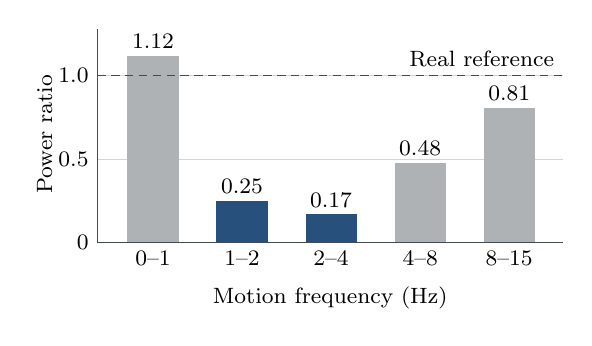
\begin{tikzpicture}[x=1.12cm,y=2.12cm,font=\footnotesize]
  \foreach \y/\value in {0/0,.5/0.5,1/1.0} {
    \draw[inkgray!24,line width=.35pt] (0,\y) -- (5.28,\y);
    \node[anchor=east,inner sep=3pt] at (0,\y) {\value};
  }
  \foreach \x/\value/\band/\shade in {
    .63/1.12/0--1/inkgray!43,1.64/.25/1--2/motionblue,
    2.65/.17/2--4/motionblue,3.66/.48/4--8/inkgray!43,4.67/.81/8--15/inkgray!43} {
    \fill[\shade] ({\x-.29},0) rectangle ({\x+.29},\value);
    \node[anchor=south,inner sep=2.4pt] at (\x,\value) {\pgfmathprintnumber[fixed,precision=2]{\value}};
    \node[anchor=north,inner sep=3pt] at (\x,0) {\band};
  }
  \draw[inkgray,thin] (0,1.28) -- (0,0) -- (5.28,0);
  \draw[inkgray,densely dashed] (0,1) -- (5.28,1);
  \node[anchor=south east,inner sep=3pt] at (5.28,1) {Real reference};
  \node at (2.64,-.33) {Motion frequency (Hz)};
  \node[rotate=90] at (-.60,.65) {Power ratio};
\end{tikzpicture}
\caption{Model A's motion power divided by real-dancer power in each frequency band, from the archived 96-window validation analysis. The dark bars mark 1--4\,Hz. Power measures how much movement occurs at those frequencies.}
\label{fig:power}
\end{figure}

\begin{figure}[t]
\centering
% Coordinates from gHO_sFM_c01_d20_mHO0_ch08, frames 60, 210, 360, and 510.
% All poses are in torso-length units with the pelvis at the cell center.
\newcommand{\drawpose}[4]{%
  \begin{scope}[shift={(#1,#2)},x=.24cm,y=-.24cm]
  #4
  \draw[#3,line width=.60pt,line cap=round,line join=round]
    (j5)--(j3)--(j1)--(j2)--(j4)--(j6)
    (j1)--(j7)--(j9)--(j11)
    (j2)--(j8)--(j10)--(j12)
    (j7)--(j8);
  \draw[#3,line width=.55pt] (j0) circle[radius=1.1pt];
  \foreach \i in {1,...,12} \fill[#3] (j\i) circle[radius=.55pt];
  \end{scope}%
}
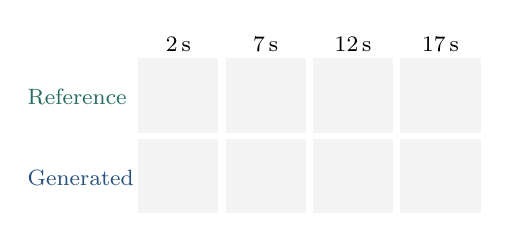
\begin{tikzpicture}[x=1cm,y=1cm,font=\footnotesize]
  \foreach \x/\seconds in {1.92/2,3.03/7,4.14/12,5.25/17} {
    \node at (\x,2.19) {\seconds\,s};
    \fill[inkgray!6] ({\x-.51},1.06) rectangle ({\x+.51},2.01);
    \fill[inkgray!6] ({\x-.51},.04) rectangle ({\x+.51},.99);
  }
  \node[anchor=west,inner sep=0pt,text=audioteal] at (0,1.52) {Reference};
  \node[anchor=west,inner sep=0pt,text=motionblue] at (0,.49) {Generated};
  \drawpose{1.92}{1.50}{audioteal}{
    \coordinate (j0) at (-0.349,-1.342);
    \coordinate (j1) at (-0.021,-1.129);
    \coordinate (j2) at (-0.583,-0.877);
    \coordinate (j3) at (0.219,-1.044);
    \coordinate (j4) at (-0.529,-0.371);
    \coordinate (j5) at (-0.203,-1.174);
    \coordinate (j6) at (-0.425,0.049);
    \coordinate (j7) at (0.188,-0.045);
    \coordinate (j8) at (-0.188,0.045);
    \coordinate (j9) at (0.283,0.690);
    \coordinate (j10) at (-0.062,0.724);
    \coordinate (j11) at (-0.444,0.790);
    \coordinate (j12) at (0.018,1.503);
  }
  \drawpose{3.03}{1.50}{audioteal}{
    \coordinate (j0) at (0.187,-1.271);
    \coordinate (j1) at (0.552,-1.090);
    \coordinate (j2) at (-0.110,-1.121);
    \coordinate (j3) at (1.007,-1.024);
    \coordinate (j4) at (-0.515,-0.950);
    \coordinate (j5) at (1.283,-1.260);
    \coordinate (j6) at (-0.594,-1.136);
    \coordinate (j7) at (0.196,0.025);
    \coordinate (j8) at (-0.196,-0.025);
    \coordinate (j9) at (-0.091,0.680);
    \coordinate (j10) at (-0.439,0.624);
    \coordinate (j11) at (0.279,1.354);
    \coordinate (j12) at (-0.430,1.325);
  }
  \drawpose{4.14}{1.50}{audioteal}{
    \coordinate (j0) at (-1.103,-0.891);
    \coordinate (j1) at (-0.784,-0.617);
    \coordinate (j2) at (-0.497,-1.106);
    \coordinate (j3) at (-0.569,-0.143);
    \coordinate (j4) at (0.024,-1.129);
    \coordinate (j5) at (-0.576,0.280);
    \coordinate (j6) at (0.398,-0.776);
    \coordinate (j7) at (-0.166,0.103);
    \coordinate (j8) at (0.166,-0.103);
    \coordinate (j9) at (-0.275,0.865);
    \coordinate (j10) at (0.069,0.376);
    \coordinate (j11) at (0.144,1.548);
    \coordinate (j12) at (0.762,0.703);
  }
  \drawpose{5.25}{1.50}{audioteal}{
    \coordinate (j0) at (-0.532,-1.240);
    \coordinate (j1) at (-0.088,-1.022);
    \coordinate (j2) at (-0.253,-1.023);
    \coordinate (j3) at (-0.032,-0.543);
    \coordinate (j4) at (-0.347,-0.810);
    \coordinate (j5) at (-0.418,-0.265);
    \coordinate (j6) at (-0.702,-0.802);
    \coordinate (j7) at (0.146,0.020);
    \coordinate (j8) at (-0.146,-0.020);
    \coordinate (j9) at (0.361,0.728);
    \coordinate (j10) at (-0.677,0.358);
    \coordinate (j11) at (0.814,1.380);
    \coordinate (j12) at (-0.148,0.818);
  }
  \drawpose{1.92}{0.49}{motionblue}{
    \coordinate (j0) at (-0.353,-1.447);
    \coordinate (j1) at (0.155,-1.118);
    \coordinate (j2) at (-0.573,-1.056);
    \coordinate (j3) at (0.526,-0.744);
    \coordinate (j4) at (-0.784,-0.645);
    \coordinate (j5) at (0.456,-0.637);
    \coordinate (j6) at (-0.820,-0.636);
    \coordinate (j7) at (0.267,0.011);
    \coordinate (j8) at (-0.243,0.018);
    \coordinate (j9) at (0.385,0.742);
    \coordinate (j10) at (-0.399,0.649);
    \coordinate (j11) at (0.410,1.174);
    \coordinate (j12) at (-0.340,1.423);
  }
  \drawpose{3.03}{0.49}{motionblue}{
    \coordinate (j0) at (-1.082,-1.176);
    \coordinate (j1) at (-0.516,-1.072);
    \coordinate (j2) at (-0.487,-0.945);
    \coordinate (j3) at (-0.448,-0.637);
    \coordinate (j4) at (-0.256,-0.371);
    \coordinate (j5) at (-0.765,-0.266);
    \coordinate (j6) at (-0.408,0.053);
    \coordinate (j7) at (0.050,-0.051);
    \coordinate (j8) at (-0.062,0.030);
    \coordinate (j9) at (-0.136,0.672);
    \coordinate (j10) at (-0.387,0.671);
    \coordinate (j11) at (0.363,1.502);
    \coordinate (j12) at (-0.145,1.465);
  }
  \drawpose{4.14}{0.49}{motionblue}{
    \coordinate (j0) at (0.208,-1.375);
    \coordinate (j1) at (0.044,-1.104);
    \coordinate (j2) at (0.136,-1.026);
    \coordinate (j3) at (-0.006,-0.686);
    \coordinate (j4) at (0.290,-0.540);
    \coordinate (j5) at (0.059,-0.362);
    \coordinate (j6) at (0.387,-0.214);
    \coordinate (j7) at (-0.004,-0.028);
    \coordinate (j8) at (-0.015,0.027);
    \coordinate (j9) at (0.119,0.584);
    \coordinate (j10) at (-0.092,0.706);
    \coordinate (j11) at (0.036,1.185);
    \coordinate (j12) at (-0.300,1.233);
  }
  \drawpose{5.25}{0.49}{motionblue}{
    \coordinate (j0) at (-0.123,-1.256);
    \coordinate (j1) at (0.254,-1.009);
    \coordinate (j2) at (-0.398,-0.941);
    \coordinate (j3) at (0.586,-0.780);
    \coordinate (j4) at (-0.620,-0.624);
    \coordinate (j5) at (0.693,-0.637);
    \coordinate (j6) at (-0.696,-0.499);
    \coordinate (j7) at (0.190,-0.009);
    \coordinate (j8) at (-0.193,0.021);
    \coordinate (j9) at (-0.002,0.540);
    \coordinate (j10) at (-0.129,0.632);
    \coordinate (j11) at (-0.083,1.300);
    \coordinate (j12) at (0.092,1.372);
  }
\end{tikzpicture}
\caption{Frames from a 20-second house validation example. The reference DWPose track and Model A generation use the same song. Poses use a common scale and are centered on the pelvis to show articulation.}
\label{fig:pose}
\end{figure}

\subsection{Step-by-step plan and measures of success}
Table~\ref{tab:plan} lists the stages in dependency order with their success measures. Stage 3 separates the factors that Run 2.1 changed together: the same losses with EDGE's training recipe, EDGE's original losses at 7.1M and 46.9M parameters (these runs are under way), then rebalancing the losses (the velocity term currently contributes about 1\% of the total) and adding regularization components one at a time. All comparisons fix model size, update budget, sampling settings, and evaluation windows, and use repeated seeds.

\textbf{Model design experiments.} Stage 4 tests architectural changes in order of cost. (1) \emph{Separate guidance:} training already drops music and genre independently, so at sampling time we combine three predictions as $\hat{x}_u + w_g(\hat{x}_g - \hat{x}_u) + w_m(\hat{x}_{gm} - \hat{x}_g)$, where equal weights reproduce the current formula; varying one weight at a time on an existing checkpoint shows whether the motion responds to the track and to the requested genre. (2) \emph{Beat-relative cross-attention:} a learned attention bias based on each motion frame's signed distance to nearby beats, in fractions of a beat, lets different heads learn anticipation, delay, and offbeat accents, in the spirit of beat-aware diffusion \cite{gao2026}; we test whether accents follow a deliberately shifted beat grid at fixed tempo, genre, and seed, reporting beat-band power alongside so that more movement alone does not count as better timing. (3) If torso variation stays high, a \emph{kinematic decoder} predicts pelvis translation and bone directions along the skeleton tree with a body scale shared across the sequence and per-frame projected-length changes, so limb lengths cannot drift while foreshortening is kept; ankle contact then gets its own supervised head. (4) If 20-second dances repeat short movements, \emph{phrase planning} predicts a coarse root path and pose anchors every few beats from the whole excerpt and conditions the five-second windows on them, following coarse-to-fine long-dance generation \cite{lodge2024}.

\textbf{Evaluation.} Kinetic and pose Fr\'echet distances (FD$_k$, FD$_p$) compare per-clip statistics of joint speed and acceleration, and of pelvis-relative joint positions and spreads, with real dances \cite{li2021}; we also report diversity, a foot-sliding proxy \cite{tseng2023}, beat-band power, and torso variation over 20\,s. For timing, we compare the share of joint acceleration within two frames of the beats with the share at phase-shifted grids, calibrated on real dances with frozen-pose and mismatched-audio controls; the standard beat-alignment score is insufficient in 2D, scoring a jittered frozen pose (0.272) above real motion (0.228). A genre classifier trained on real motion scores samples that share audio but differ in requested genre. Final numbers are computed once, on the held-out songs, after all settings are fixed.

\textbf{Team responsibilities.} YinHsuan Hsu leads pose and audio processing, data audits, and the pose-estimator study. Sizhe Zhang leads the baseline and diffusion models, cloud training, and ablations. Yi Xin leads the evaluation metrics, held-out testing, and visualization. All members review the demo and prepare the report and poster.

\section{Feasibility and Limitations}
\textbf{Endpoint.} The semester goal is an evaluated 2D generator with a music-synchronized demo; the data, training, evaluation, and rendering code already exist. We stop at 2D because the four-week schedule and our compute (single 24\,GB GPUs; a 30,000-update run takes about 45 minutes for the 7.1M model and 1.75 hours for the 46.9M model) leave room to solve the rhythm--stability trade-off, but not to also build a 3D pipeline. Rendering meshes and simulating physics are out of scope. If time allows, we will load the AIST++ 3D annotations \cite{li2021} as a first step toward 3D.

\textbf{Challenges and initial solutions.}
\begin{itemize}
\item \emph{Damped, averaged motion:} energy loss, larger model, longer training; monitored by speed and beat-band power.
\item \emph{Body-size drift in 2D:} dancer-level scaling and the bone-length loss; restricting the energy term to speed if its amplitude part enlarges limbs.
\item \emph{Overfitting with 3.7 training hours:} basic dances, time-stretch and geometric augmentation, checkpoint selection on validation data.
\item \emph{Training instability:} the 46.9M model diverged within 500 updates at batch size 64; warm-up and gradient clipping fixed it.
\item \emph{Noisy 2D labels:} occlusion and foreshortening in breaking and turns; validity masks, smoothing, and per-frame bone targets.
\end{itemize}

\textbf{Limitations that need investigation.} We do not yet know whether higher beat-band power is perceived as better timing, whether validation loss selects the checkpoints with the best dances (beat-level movement kept improving after it stopped), whether the model follows the genre label when the music suggests another genre, how it handles music with variable tempo or weak beats, and whether differences between pose estimators survive training. Earlier demos used some held-out songs; we document this and lock all settings before final scoring.

\balance
\section{Potential Impact}
Beat2Body could help choreographers compare movement ideas over the same musical phrase and give animation and game teams quick reference motion for blocking scene timing; skeletons can be retargeted to characters or used for motion editing. Because it learns from single-camera video, the approach extends to dance styles and performers never captured in a studio, and to other music-paced movement such as fitness and rehabilitation exercises. The pose-estimator comparison will show which tool to use when collecting motion data from video, and the beat-band and phase-shift tests offer reusable rhythm checks for other music-conditioned motion tasks, such as gesture generation for speech and music.

\begin{thebibliography}{99}

\bibitem{lee2019}
H.-Y. Lee \emph{et al.}, \textquotedblleft\href{https://proceedings.neurips.cc/paper_files/paper/2019/hash/7ca57a9f85a19a6e4b9a248c1daca185-Abstract.html}{Dancing to music},'' in \emph{Advances in Neural Information Processing Systems}, vol. 32, 2019.

\bibitem{li2021}
R. Li, S. Yang, D. A. Ross, and A. Kanazawa, \textquotedblleft\href{https://openaccess.thecvf.com/content/ICCV2021/html/Li_AI_Choreographer_Music_Conditioned_3D_Dance_Generation_With_AIST_ICCV_2021_paper.html}{AI Choreographer: Music conditioned 3D dance generation with AIST++},'' in \emph{Proc. IEEE/CVF ICCV}, 2021, pp. 13401--13412.

\bibitem{tseng2023}
J. Tseng, R. Castellon, and C. K. Liu, \textquotedblleft\href{https://openaccess.thecvf.com/content/CVPR2023/html/Tseng_EDGE_Editable_Dance_Generation_From_Music_CVPR_2023_paper.html}{EDGE: Editable dance generation from music},'' in \emph{Proc. IEEE/CVF CVPR}, 2023, pp. 448--458.

\bibitem{gao2026}
Y. Gao, Q. Wu, S. Zhu, K. He, W. Weng, and J. Zhou, \textquotedblleft\href{https://doi.org/10.3390/info17080808}{ChoreDiffusion: Beat-aware diffusion for music-to-dance generation},'' \emph{Information}, vol. 17, no. 8, Art. no. 808, 2026.

\bibitem{dancedit}
Y. Zhang, H. Zou, L. Feng, C. Xie, R. Yu, and Z. Zhan, \textquotedblleft\href{https://arxiv.org/abs/2512.11720}{Reframing music-driven 2D dance pose generation as multi-channel image generation},'' arXiv:2512.11720, 2025.

\bibitem{tsuchida2019}
S. Tsuchida, S. Fukayama, M. Hamasaki, and M. Goto, \textquotedblleft\href{https://archives.ismir.net/ismir2019/paper/000060.pdf}{AIST Dance Video Database: Multi-genre, multi-dancer, and multi-camera database for dance information processing},'' in \emph{Proc. ISMIR}, 2019.

\bibitem{aistdownload}
National Institute of Advanced Industrial Science and Technology, \textquotedblleft AIST Dance Video Database.'' [Online]. Available: \href{https://aistdancedb.ongaaccel.jp/database_download/}{Download index} and \href{https://aistdancedb.ongaaccel.jp/terms_of_use/}{terms of use}.

\bibitem{beat2bodydata}
Beat2Body Team, \textquotedblleft AIST Dance 2D keypoints,'' dataset cards, 2026. [Online]. Available: \href{https://huggingface.co/datasets/SizheZ03/AISTDance_dwpose}{DWPose}, \href{https://huggingface.co/datasets/SizheZ03/AISTDance_openpose}{OpenPose}, and \href{https://huggingface.co/datasets/SizheZ03/AISTDance_mediapipe}{MediaPipe}.

\bibitem{yang2023}
Z. Yang, A. Zeng, C. Yuan, and Y. Li, \textquotedblleft\href{https://arxiv.org/abs/2307.15880}{Effective whole-body pose estimation with two-stages distillation},'' in \emph{Proc. IEEE/CVF ICCV Workshops}, 2023.

\bibitem{cao2021}
Z. Cao, G. Hidalgo, T. Simon, S.-E. Wei, and Y. Sheikh, \textquotedblleft\href{https://doi.org/10.1109/TPAMI.2019.2929257}{OpenPose: Realtime multi-person 2D pose estimation using part affinity fields},'' \emph{IEEE Trans. Pattern Anal. Mach. Intell.}, vol. 43, no. 1, pp. 172--186, 2021.

\bibitem{bazarevsky2020}
V. Bazarevsky \emph{et al.}, \textquotedblleft\href{https://arxiv.org/abs/2006.10204}{BlazePose: On-device real-time body pose tracking},'' arXiv:2006.10204, 2020.

\bibitem{beat2bodyprogress}
Beat2Body Team, \textquotedblleft\href{https://github.com/novaz03/beat2body/tree/cb66cc7b4f78f4409baee615d14b34a6879790ec/reports/2026-11-19_progress}{2D music-to-dance progress report and archived validation metrics},'' Nov. 19, 2026.

\bibitem{song2021}
J. Song, C. Meng, and S. Ermon, \textquotedblleft\href{https://arxiv.org/abs/2010.02502}{Denoising diffusion implicit models},'' in \emph{Proc. ICLR}, 2021.

\bibitem{salimans2022}
T. Salimans and J. Ho, \textquotedblleft\href{https://arxiv.org/abs/2202.00512}{Progressive distillation for fast sampling of diffusion models},'' in \emph{Proc. ICLR}, 2022.

\bibitem{lodge2024}
R. Li \emph{et al.}, \textquotedblleft\href{https://openaccess.thecvf.com/content/CVPR2024/html/Li_Lodge_A_Coarse_to_Fine_Diffusion_Network_for_Long_Dance_CVPR_2024_paper.html}{Lodge: A coarse to fine diffusion network for long dance generation guided by the characteristic dance primitives},'' in \emph{Proc. IEEE/CVF CVPR}, 2024.

\end{thebibliography}
\end{document}
